\section{Introduzione}
Lo scopo di questo progetto consiste nella classificazione dell'attività fisica svolta da un individuo grazie a delle misure ottenute con una board Arduino Nano 33 BLE Sense posizionata sopra la caviglia di un soggetto. Dopo essersi connessi alla board tramite BLE e in base al firmware caricato sull'Arduino, è possibile utilizzare l'applicazione in due modalità:
\begin{itemize}
	\item modalità acquisizione dati: l'applicazione riceve e salva i dati inviati dalla piattaforma;
	\item modalità activity tracker: l'applicazione visualizza la predizione dell'attività che il soggetto sta svolgendo (camminata, cyclette, salto con la corda oppure l'individuo è fermo).
\end{itemize}
Sono stati utilizzati i seguenti sensori presenti sulla board:
\begin{itemize}
	\item accelerometro triassiale; 
	\item giroscopio triassiale;
	\item sensore di temperatura e di umidità.
\end{itemize}
Tuttavia, i dati di temperatura e umidità non sono stati utilizzati poiché i dati ricavati non si sono mostrati essere significativi per l'obiettivo di questo progetto. \`E stata inoltre modificata la libreria che gestisce la comunicazione con la IMU presente sul BLE (file \texttt{LSM9DS1.cpp}) per modificare il fondo scala dell'accelerometro (che di default è impostato a 4g):
\begin{itemize}
	\item accelerometro: fondo scala 8g, frequenza di campionamento \SI{119}{\hertz};
	\item giroscopio: fondo scala 2000 dps, frequenza di campionamento \SI{119}{\hertz}.
\end{itemize}

Per l'attività di classificazione dell'attività si è scelto di utilizzare un approccio \textit{black-box}, utilizzando una rete neurale opportunamente allenata con i dati raccolti dalla board. La rete neurale, sviluppata tramite il framework Edge Impulse, è stata poi installata sull'Arduino. Utilizzando quindi un modello di \textit{edge computing}, è stato possibile realizzare una applicazione, sviluppata grazie al framework Qt, che si occupa solamente della visualizzazione dei dati e della predizione dell'attività svolta. In questo modo, si è potuto mantenere una frequenza di campionamento dei dati relativamente alta (circa \SI{66}{\hertz}) senza sovraccaricare la comunicazione BLE.
\todo{se riesco questo weekend misuro la corrente assorbita con un tester}
\section{Acquisizione dei dati}
\todo{mettere foto posizione arduino su gamba}
\todo{inserire foto schermata di acquisizione}
Per poter acquisire i dati con Arduino, è stato necessario sviluppare un firmware apposito che consentisse di inviare le acquisizioni utilizzando la tecnologia Bluetooth Low Energy (BLE), in cui l'Arduino è stato utilizzato nel ruolo di \textit{peripheral} mentre l'applicazione assume il ruolo di \textit{central}. La board di Arduino espone un servizio su cui viene scritta una caratteristica che contiene i dati delle misure. Il central viene notificato ogniqualvolta che il \textit{peripheral} aggiorna la caratteristica e ne legge il contenuto il quale viene salvato su un file .csv.

Inizialmente, si è cercato di utilizzare una frequenza di campionamento dei dati pari a \SI{100}{\hertz}. Tuttavia, si è verificato che il flusso di dati non era sostenibile dal BLE. Tramite delle prove si è poi stabilito che una frequenza di campionamento dei dati sostenibile era di circa \SI{66}{\hertz} (un campione ogni \SI{15}{\milli\second}). Per assicurare una buona precisione nella frequenza di campionamento, si è scelto di utilizzare il meccanismo degli interrupt (Interrupt Service Routine), in cui un funzione di callback venie chiamata ogni \SI{15}{\milli\second}. Infatti, non è possibile utilizzare la funzione \textit{delay}, che non garantisce intervalli regolari di acquisizione. Inoltre, ciò permette di realizzare una applicazione \textit{pseudo} concorrente, in cui la funzione \textit{loop} principale si occupa dell'invio dei dati tramite BLE, mentre un'altra funzione, attivata da un interrupt, si occupa di acquisire i dati. Ciò però non si è mostrato sufficiente a garantire un frequenza di campionamento accurata in quanto si è visto che il tempo necessario all'invio dei dati tramite BLE non è costante e portava alla perdita di alcuni dati.
Per questo motivo, è stato introdotto un buffer circolare tramite la libreria \url{https://github.com/rlogiacco/CircularBuffer}. In questo modo, se la comunicazione subisce un ritardo non si ha perdita dei dati. Di seguito si riportano un esempio dei dati dell'accelerometro e giroscopio ottenuti durante una camminata di un soggetto (\Fig\ref{fig:imu_data}).
\begin{figure}[tbh]
	\centering
	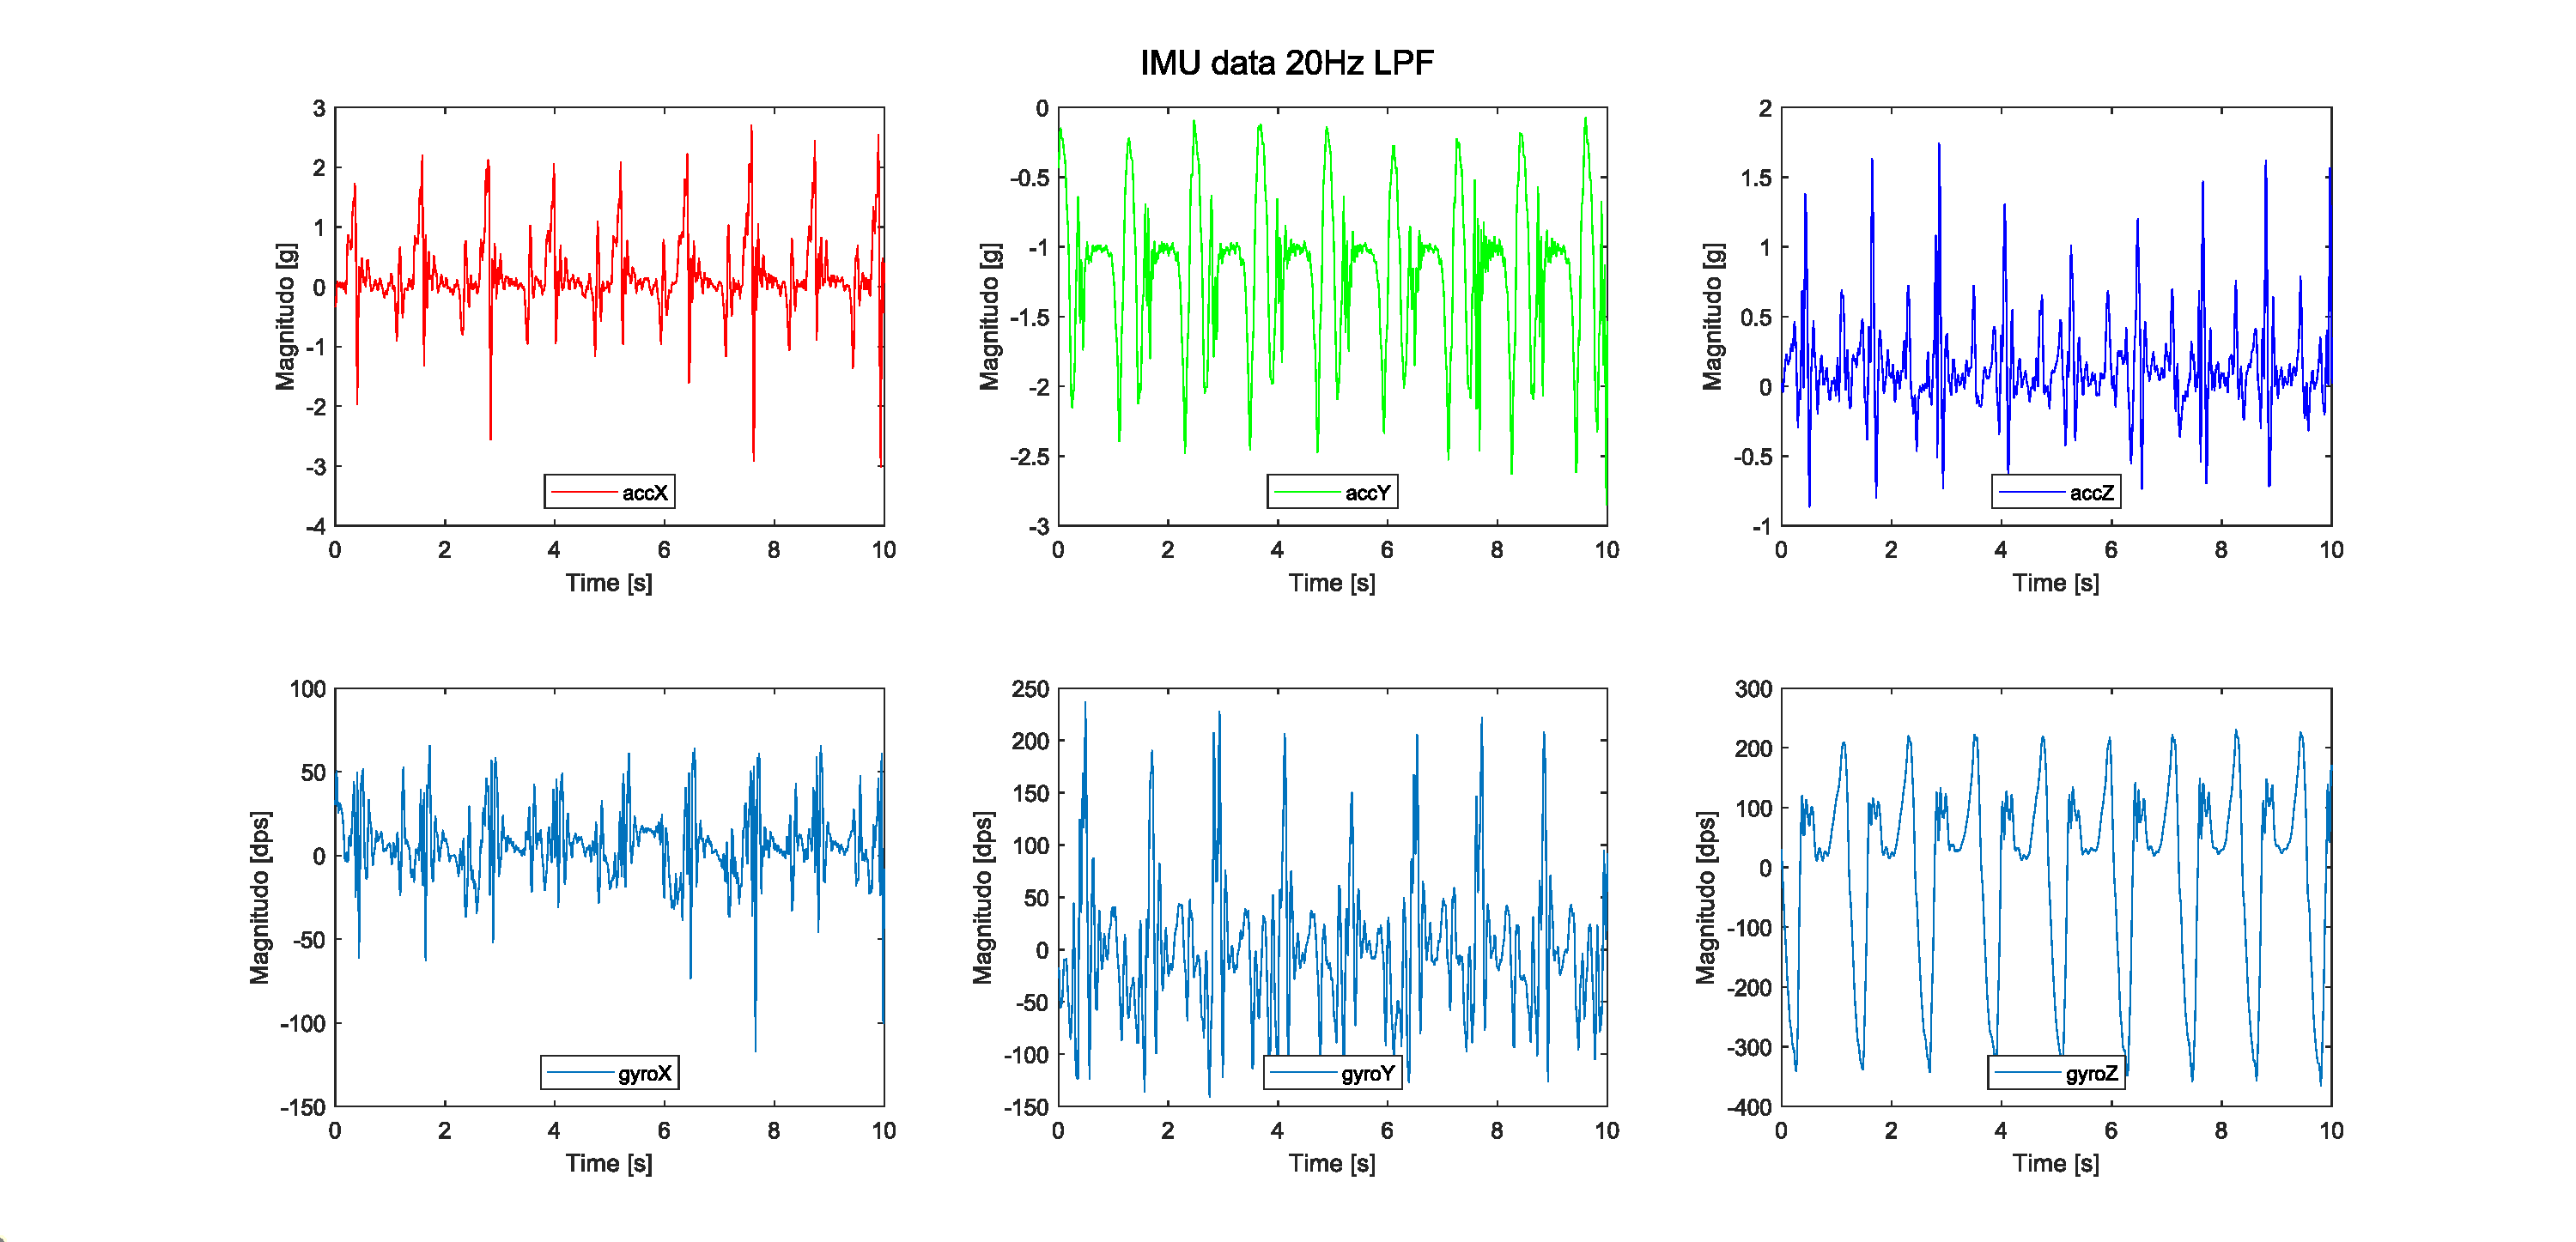
\includegraphics[width=1\linewidth]{./ImageFiles/IMU_data_example.pdf}
	\caption{Dati acquisiti dall'accelerometro e giroscopio durante una camminata. I dati sono campionati ogni \SI{15}{\milli\second} e sono stati filtrati con un filtro passa basso con frequenza di taglio di \SI{20}{\hertz}.}
	\label{fig:imu_data}
\end{figure}
Nella figura \ref{fig:time_interval}a) sono rappresentati gli intervalli di tempo tra due acquisizioni successive su una misura di \SI{76}{\second}. Il tempo medio risultate è di \SI{15.0057}{\milli\second} con una deviazione standard di \SI{0.4405}{\milli\second}. Senza buffer circolare (\Fig\ref{fig:time_interval}b)) si ottiene una media di circa \SI{16.1630}{\milli\second} con una deviazione standard di \SI{6}{\milli\second}. Infatti, è possibile vedere nell'immagine che si hanno molti più outliner.
Si tenga in considerazione che l'istante di tempo in cui si eseguiva l'acquisizione è stato misurato con la funzione \textit{millis()}, che ha errore di $\pm \SI{1}{\milli\second}$. 
\begin{figure}[tbh]
	\centering
	a)
	\begin{minipage}{.900\textwidth}
		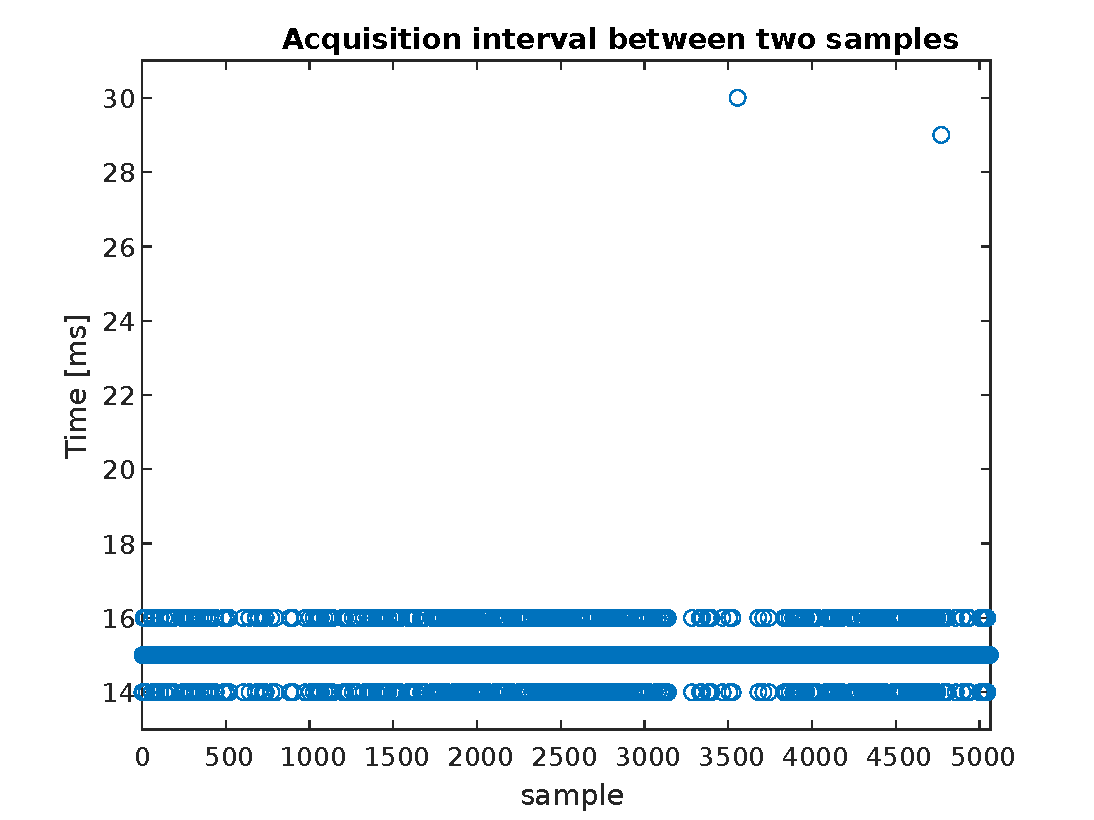
\includegraphics[width=0.8\linewidth]{./ImageFiles/interval_time.pdf}
	\end{minipage}
	\\b)
	\begin{minipage}{.900\textwidth}
		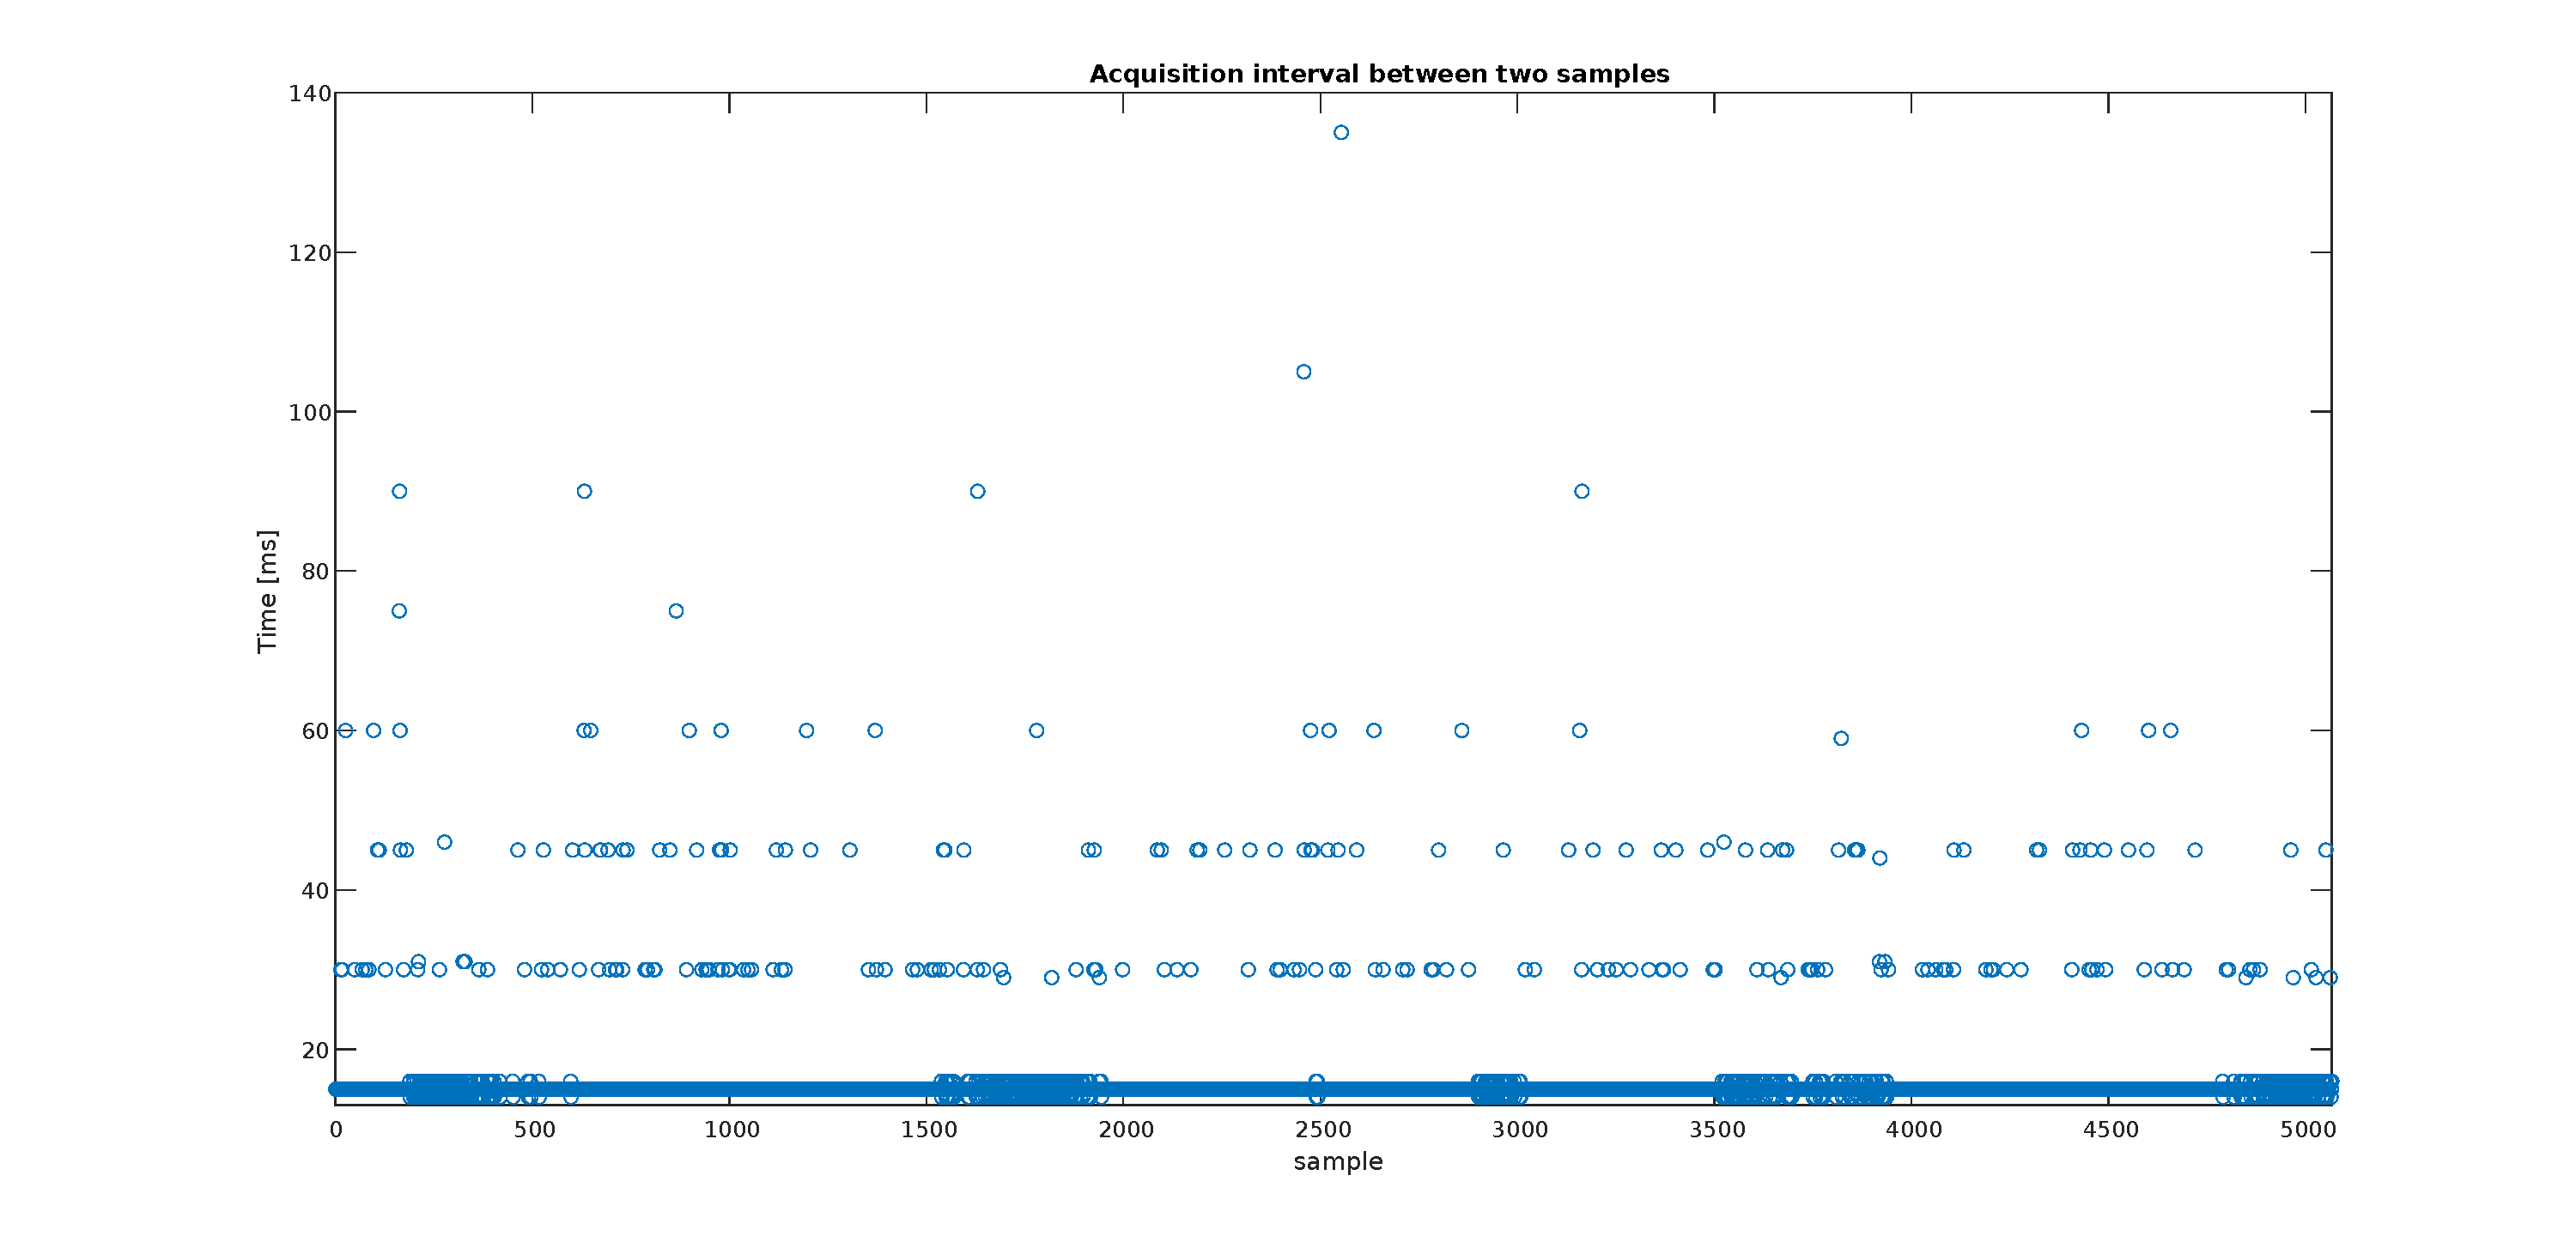
\includegraphics[width=\linewidth]{./ImageFiles/interval_time_2}
	\end{minipage}
	\caption{Tempo tra due campioni successivi su una acquisizione di \SI{76}{\second}: a) con buffer circolare, b) senza buffer circolare}
	\label{fig:time_interval}
\end{figure}

\section{Classificazione delle attività}

\todo{inserirei qui un po una minima spiegazione dei dati... tipo che quale asse è migliore, su quale si vede meglio i passi e cosi}
\todo{I dati acquisisti sono stati caricati su Edge Impulse. Come è stato creato l'impulse. Su cosa lavora. Cosa produce edge impulse. Come son state modificate le finestre. Feature spettrali. Bontà del modello e testing.}

Per realizzare la classificazione e poi visualizzarla sull'applicazione è stato sviluppato un ulteriore firmware, al cui interno sono stati creati due thread differenti. Nel primo vengono acquisiti i dati dai sensori fino a quando il buffer non risulta pieno, mentre nel secondo si aggiorna il collegamento BLE in modo da poter trasmettere successivamente la previsione della classificazione. Una volta che il buffer è pieno si estraggono i suoi elementi tramite Digital Signal Processing in modo da convertire il buffer in un segnale, che viene poi passato al classificatore per fare inferenza. La realizzazione concreta della classificazione prevede di richiamare le librerie di Edge Impulse. Infine il risultato della classificazione viene trasmesso tramite una caratteristica su BLE all'applicazione, che mostra a video l'immagine relativa all'attività fisica rilevata. Le possibili schermate visualizzate sull'applicazione si distinguono in base all'attività come mostrato nella figura \ref{fig:attivitafisica}.

\begin{figure}[tbh]
	\centering
	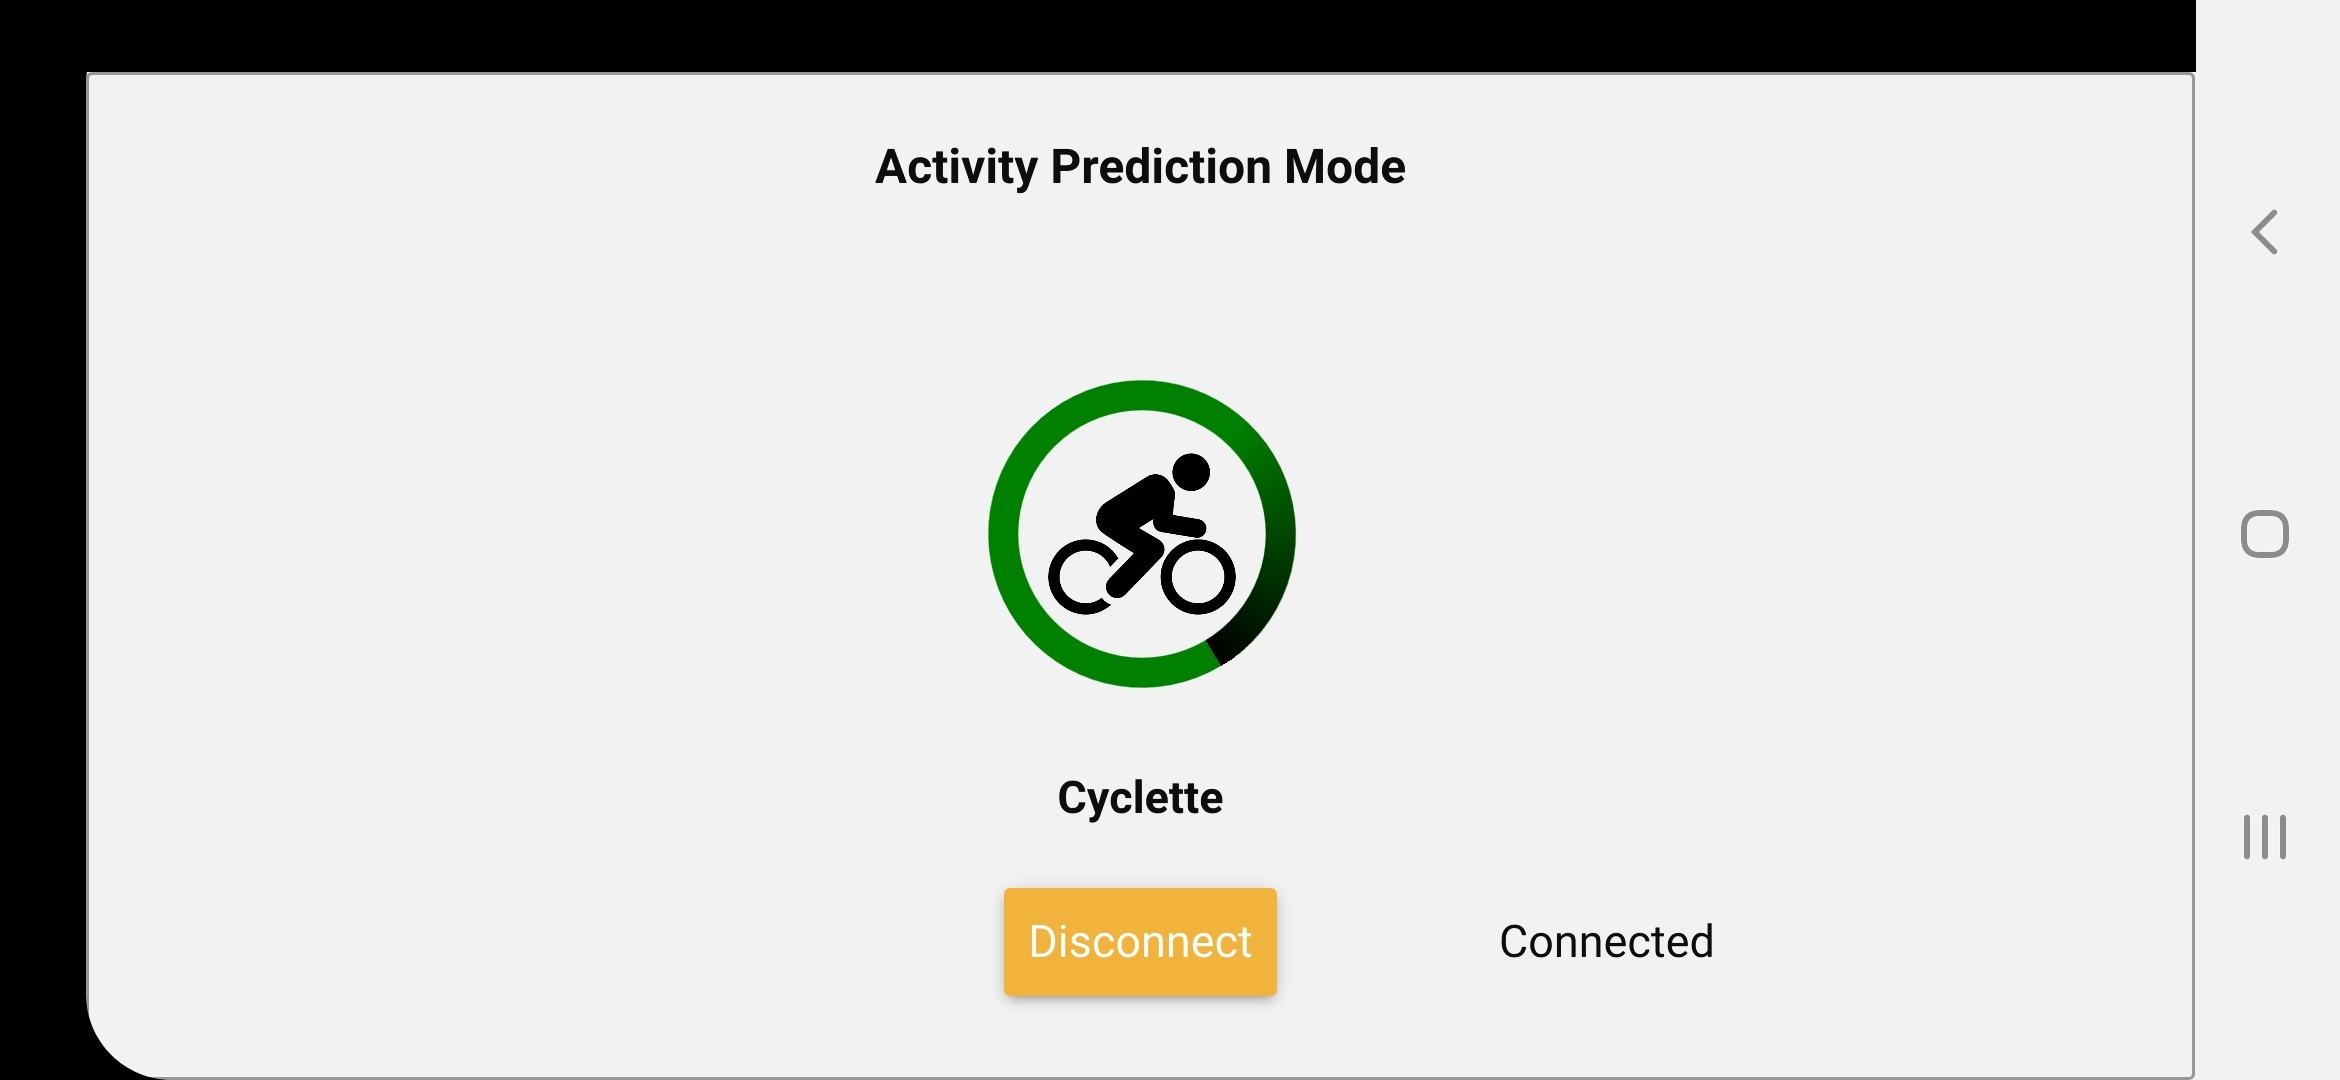
\includegraphics[width=0.4\linewidth]{./ImageFiles/cyclette}
	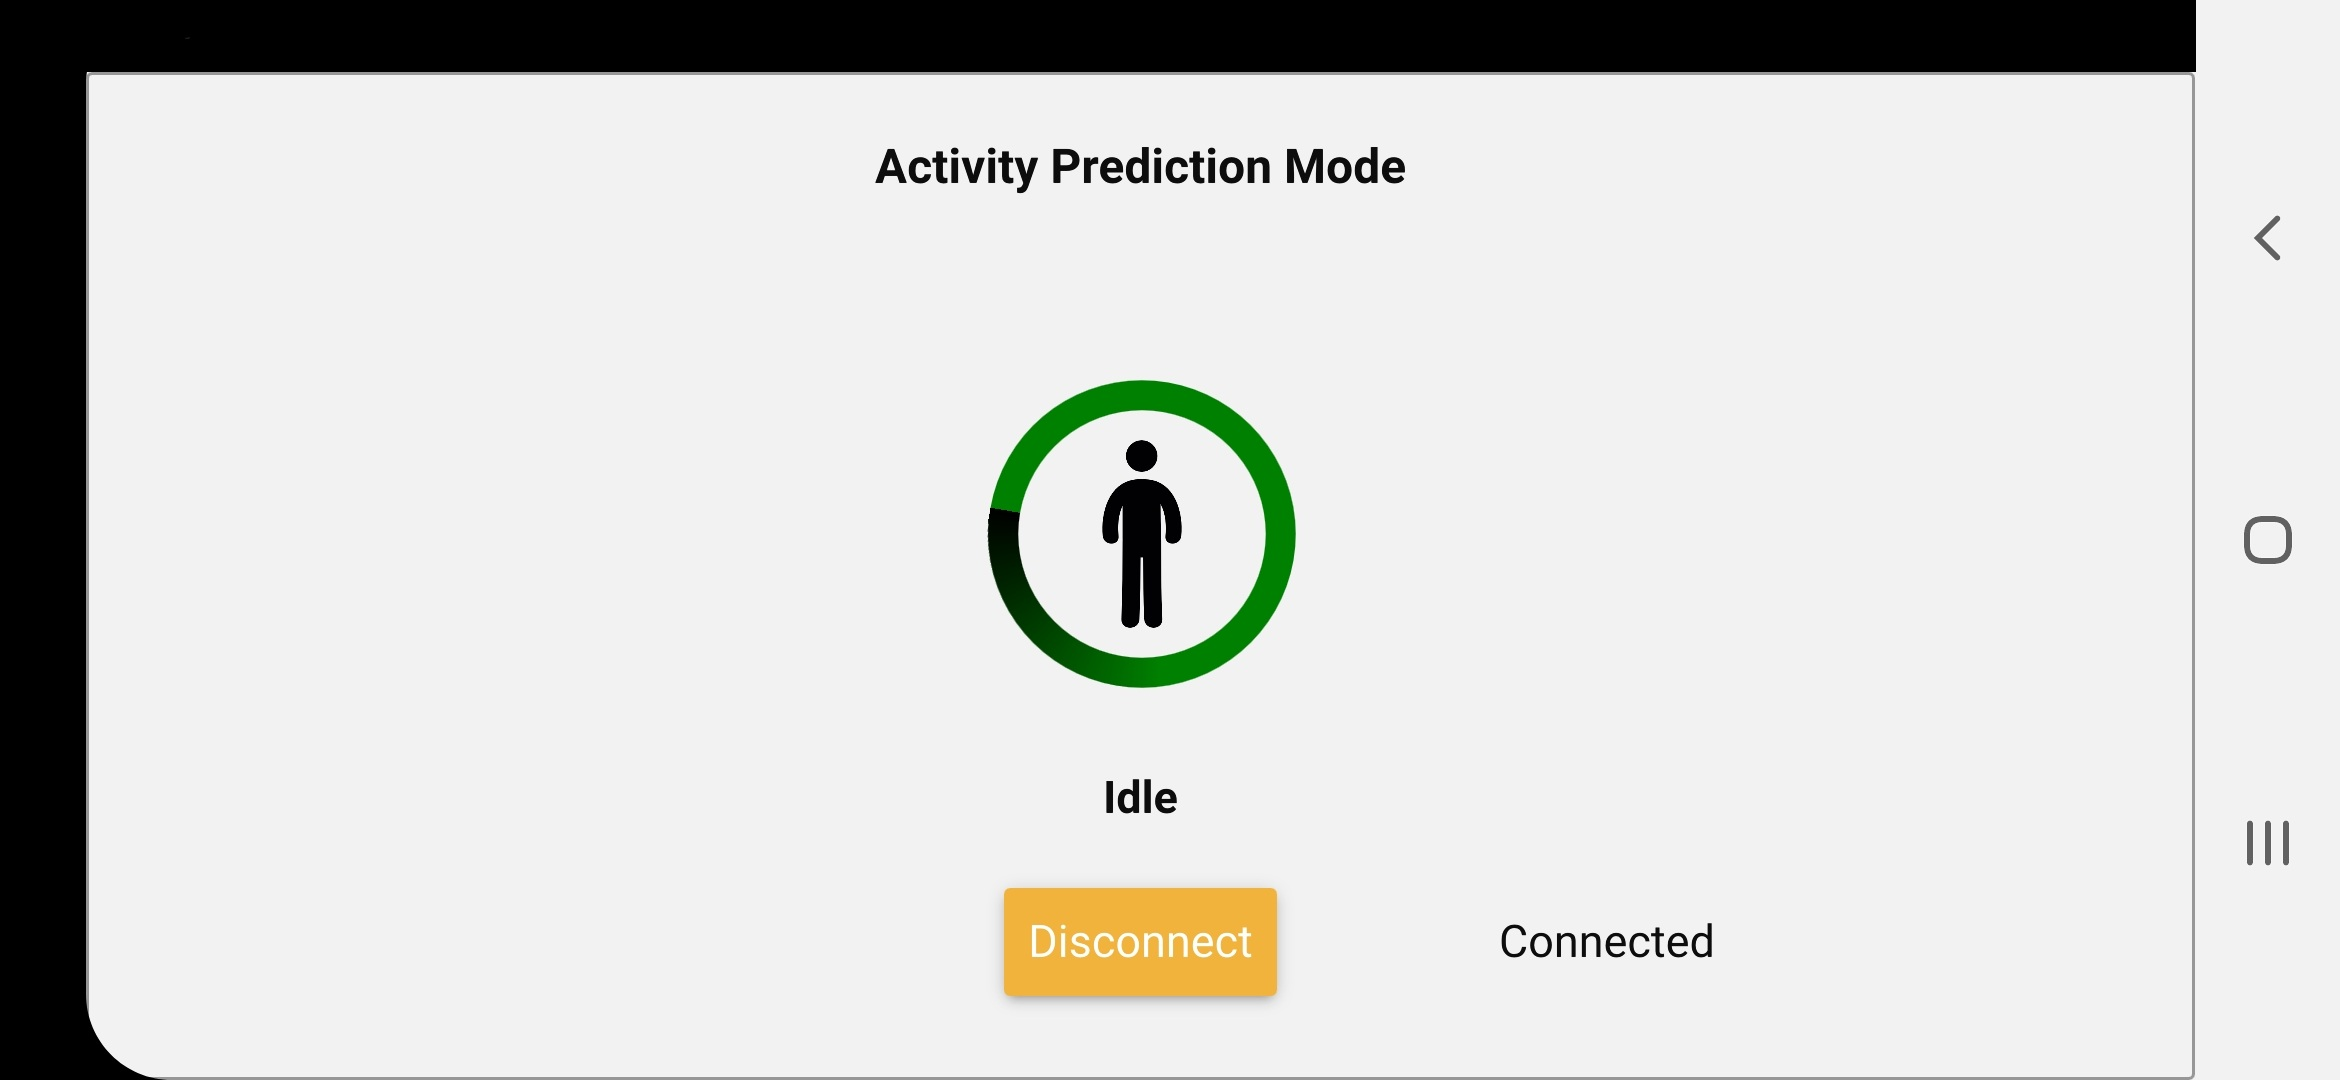
\includegraphics[width=0.4\linewidth]{./ImageFiles/idle}
	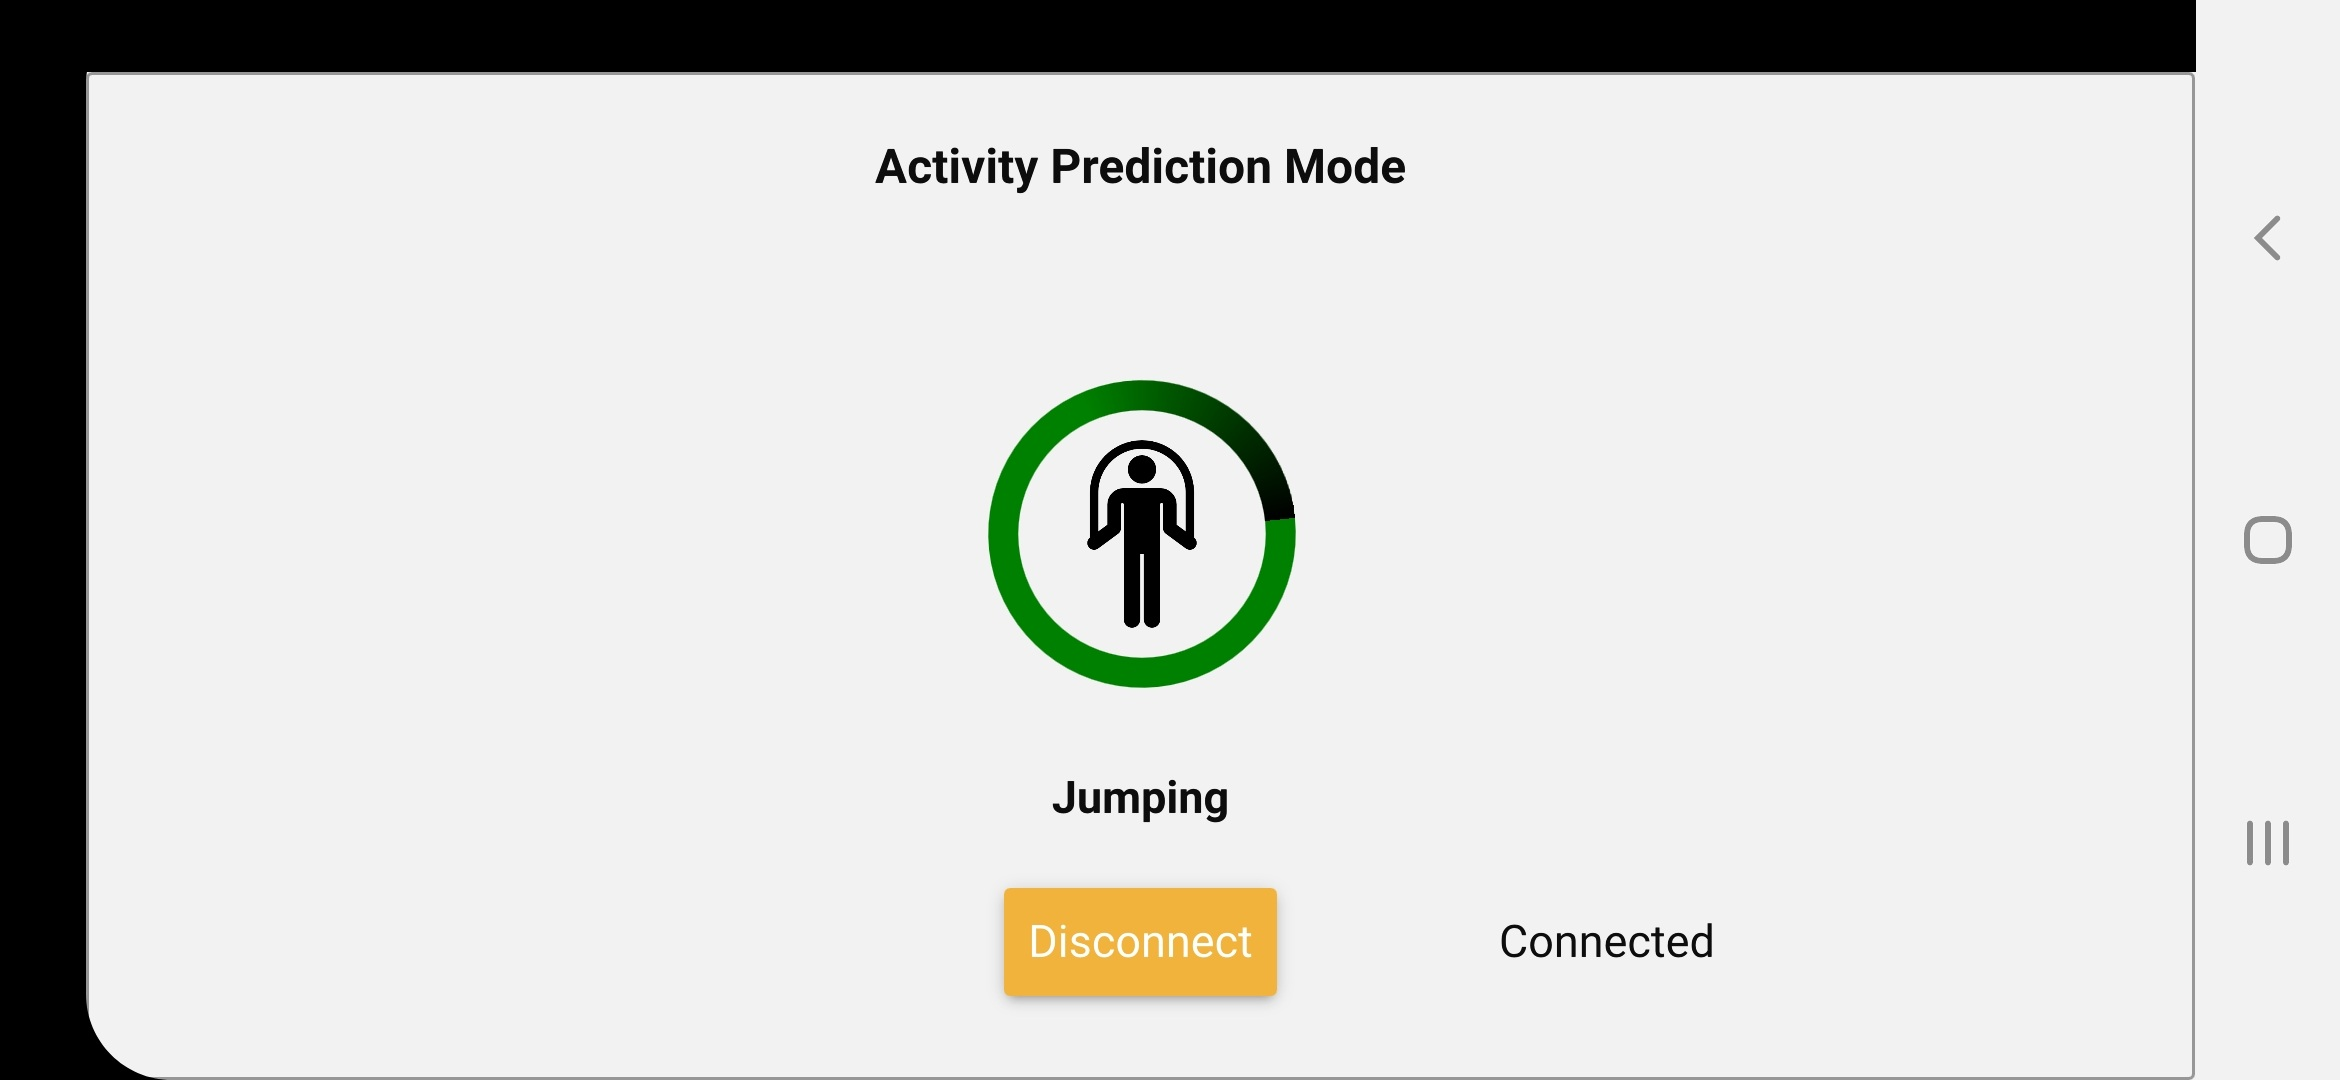
\includegraphics[width=0.4\linewidth]{./ImageFiles/jumping}
	%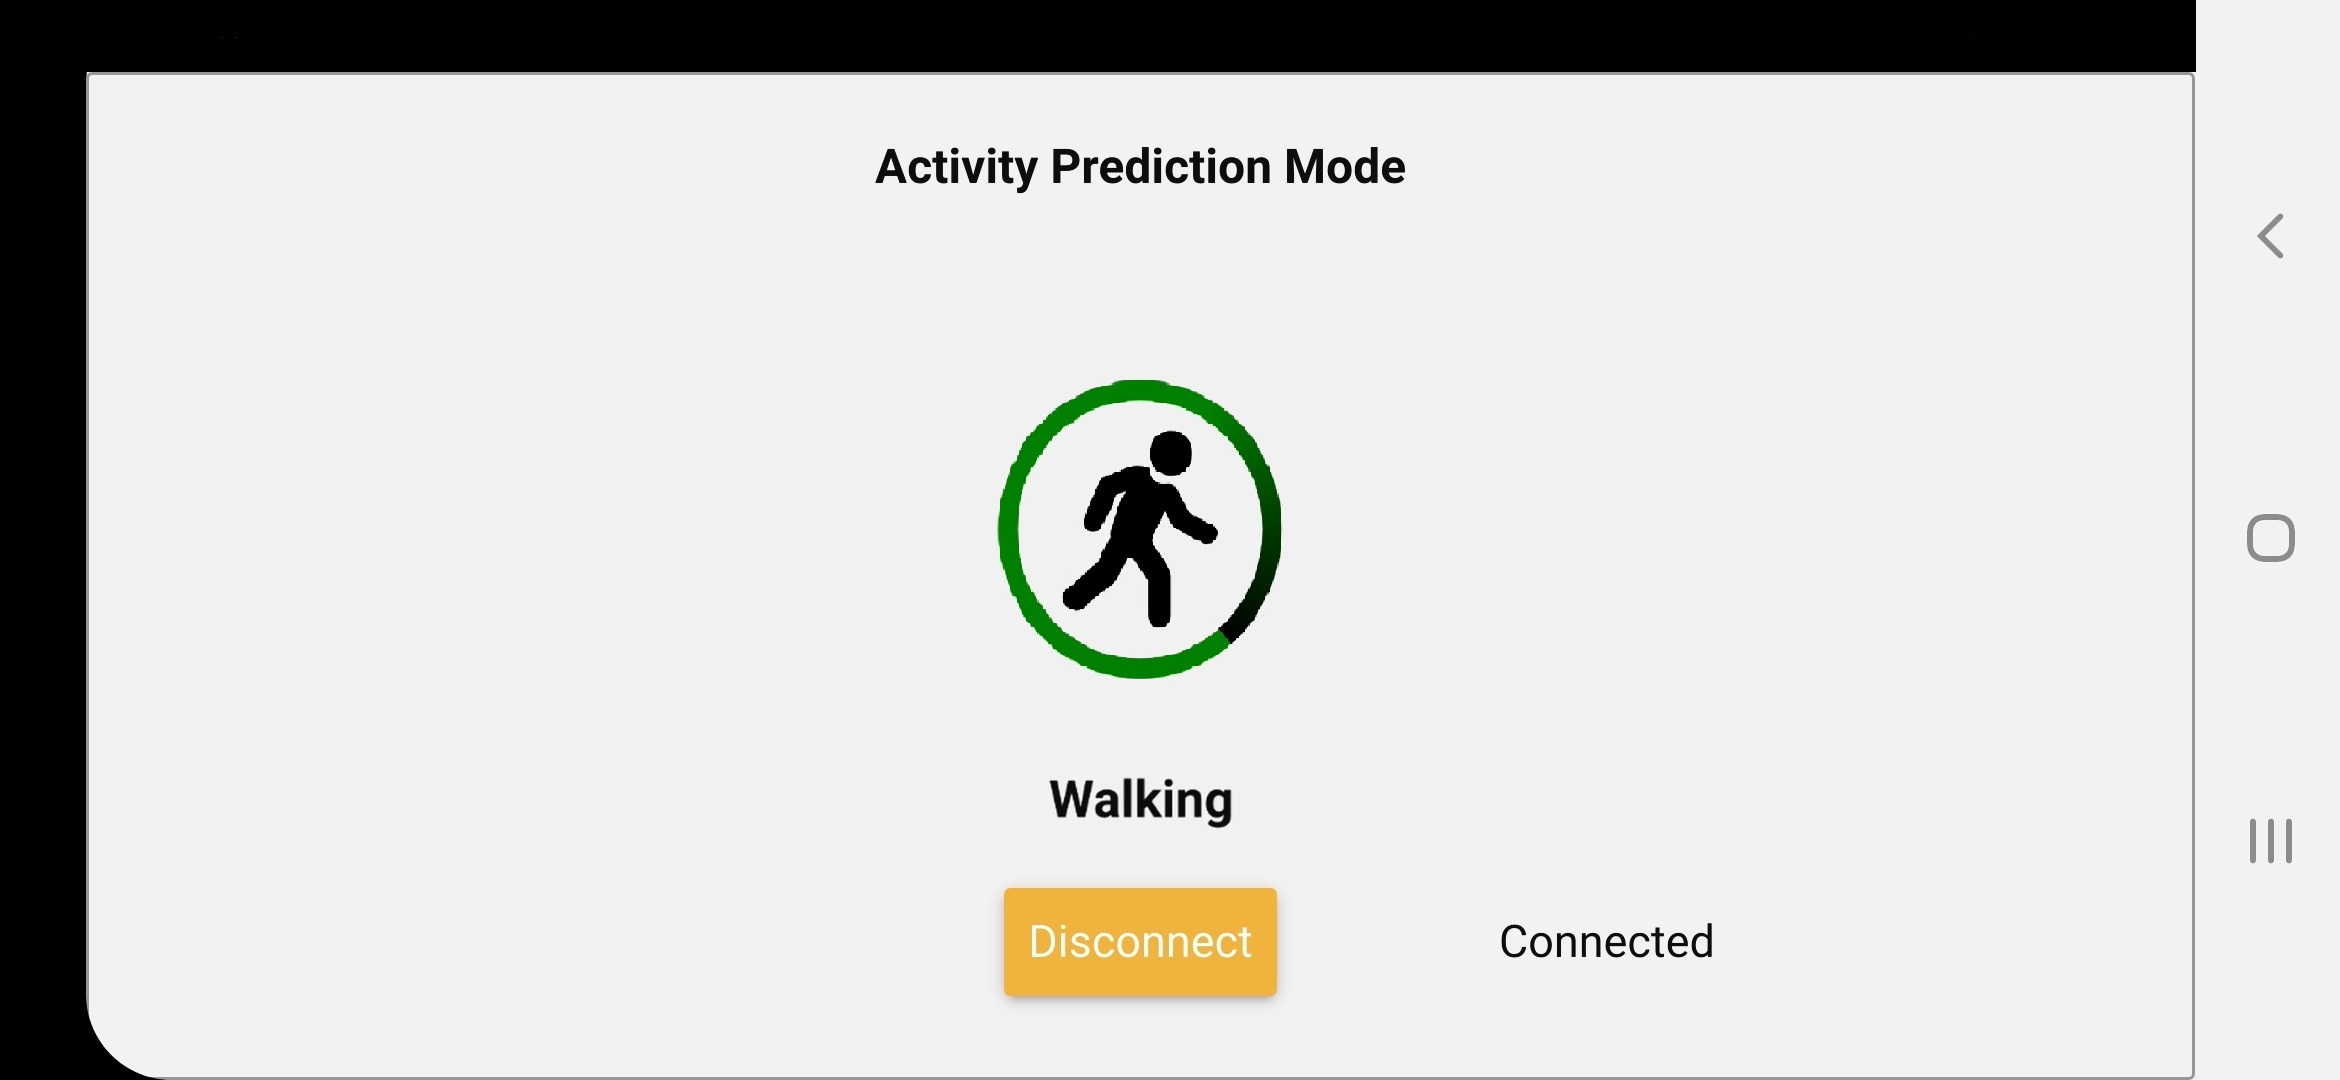
\includegraphics[width=0.4\linewidth]{./ImageFiles/walking}
	\caption{Schermate per le possibili attività: cyclette, fermo, salto della corda e camminata.}
	\label{fig:attivitafisica}
\end{figure}
\todo{manca schermata walking}

Invece nei momenti in cui non si riesce a classificare l'attività in corso in nessuna di quelle possibili si visualizza la schermata della figura \ref{fig:attesa}.

\begin{figure}[tbh]
	\centering
	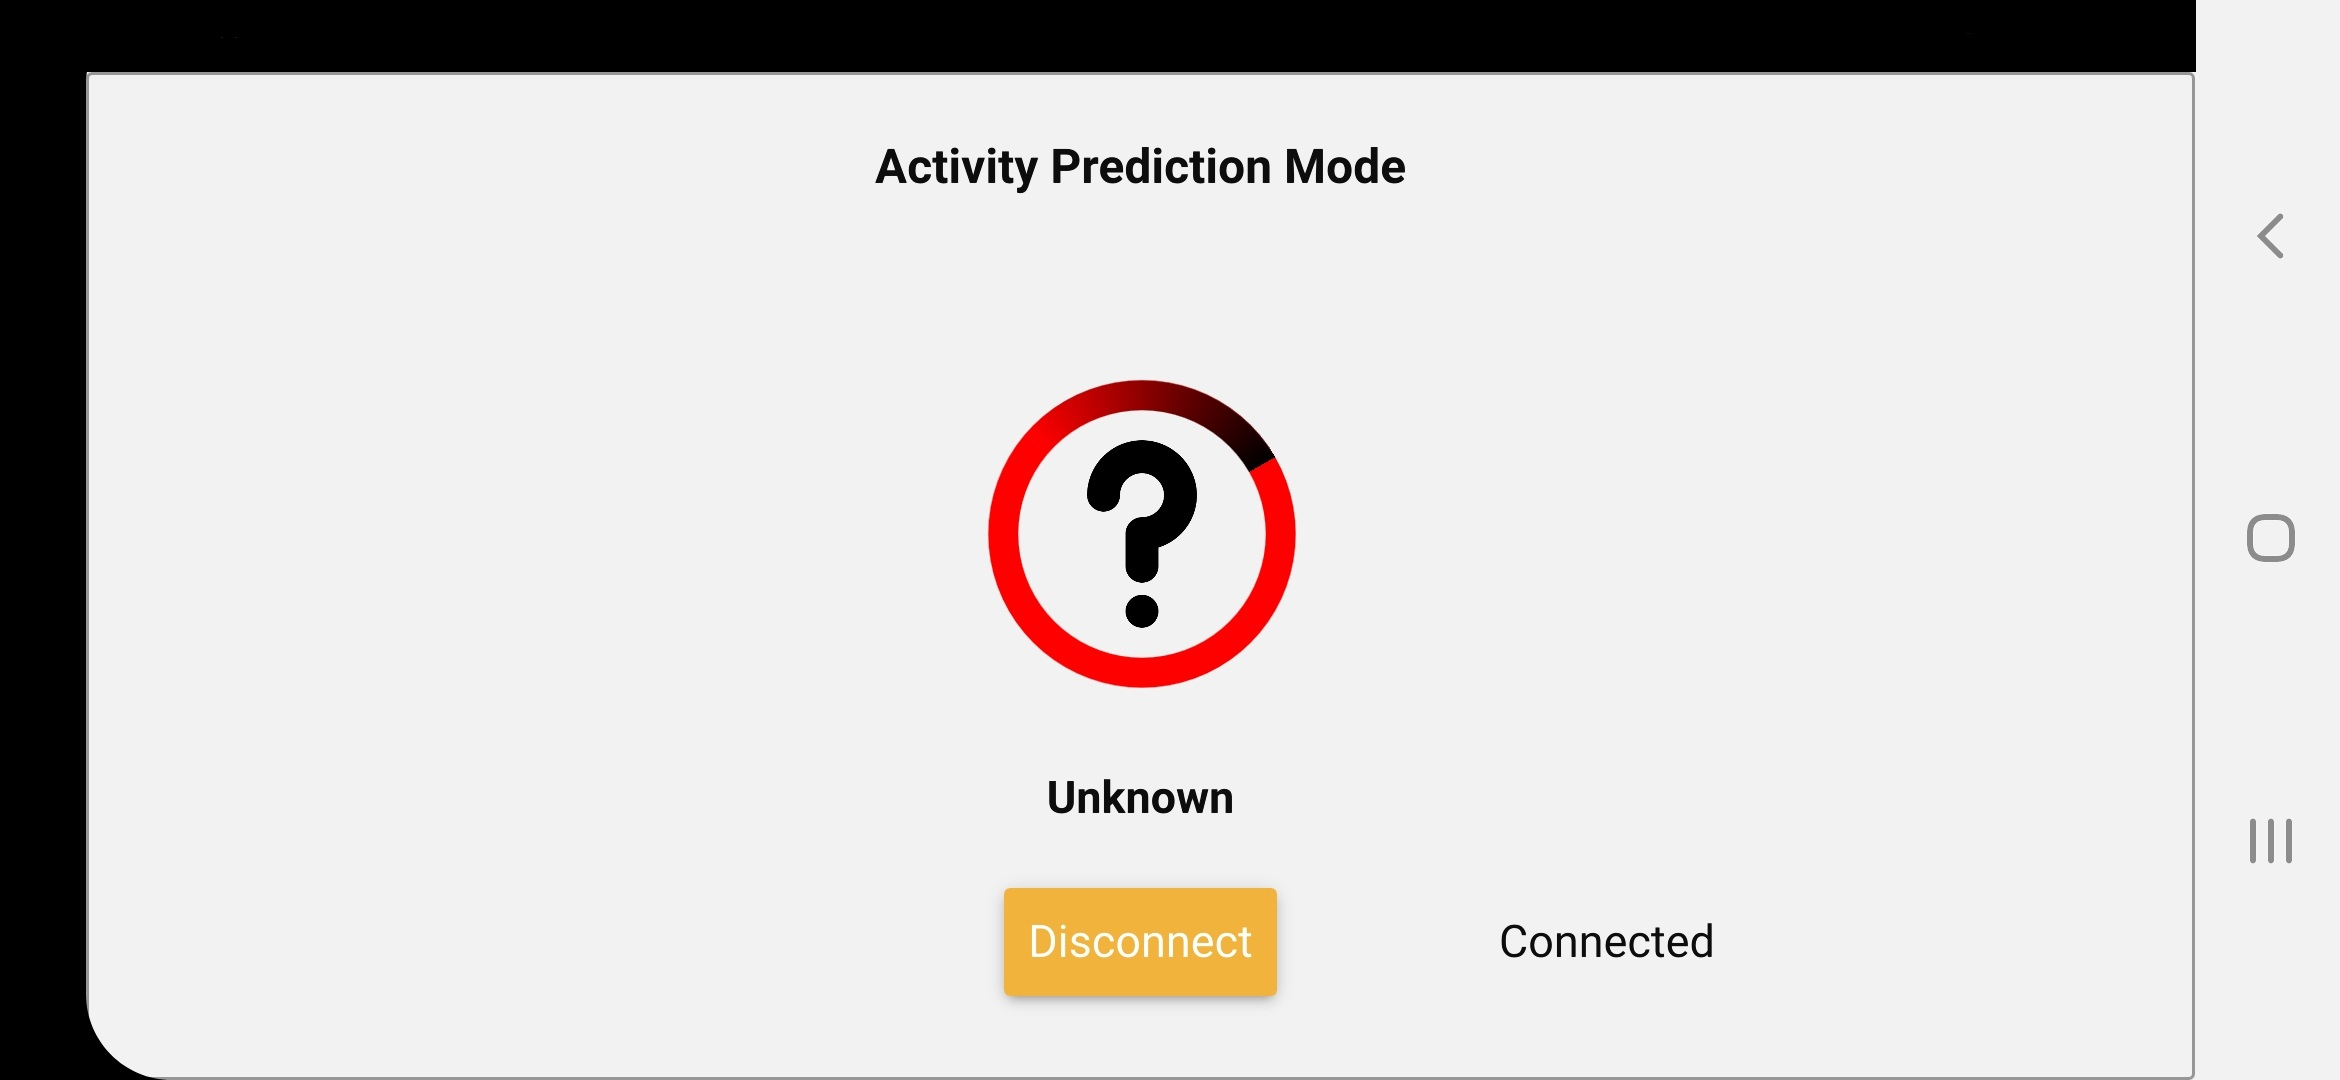
\includegraphics[width=0.4\linewidth]{./ImageFiles/unknown}
	\caption{Schermata per le attese precedenti la classificazione o per misure non classificabili.}
	\label{fig:attesa}
\end{figure}

\todo{Quali sono i tempi che impiega il firmware. Per passare da una attività all'altra servono circa tot secondi perchè si deve svuotare il buffer.}